\documentclass{article}
\usepackage[utf8]{inputenc}

\usepackage{tikz}
\usetikzlibrary{positioning, fit}

\usepackage{geometry}
\geometry{
margin=10mm,
}

\begin{document}

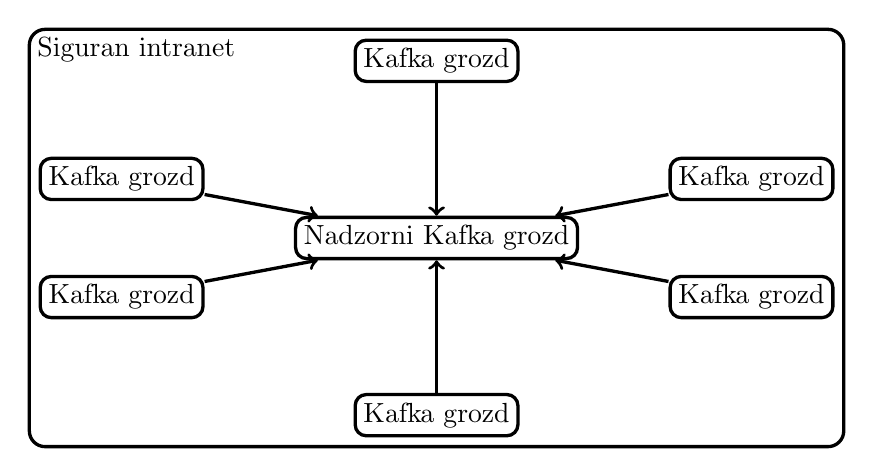
\begin{tikzpicture}[ % has a lot of options; consult the pgf manual
bend angle=15,
long_square/.style={rectangle, draw=black, fill=white, very thick, inner sep=3pt, minimum width=14mm},
rounded_square/.style={rectangle, rounded corners, draw=black, fill=white, very thick, inner sep=3pt, minimum width=14mm},
empty_circle/.style={rectangle, rounded corners=2mm, draw=black, fill=white, very thick, minimum size=4mm},
point/.style={circle, inner sep=0mm},
fit_square/.style={rectangle, rounded corners=2mm, draw=black, very thick},
both_arrow/.style={<->, very thick},
out_arrow/.style={->, very thick},
in_arrow/.style={<-, very thick},
dashed_arrow/.style={loosely dashed, very thick},
above_edge_text/.style={above, midway, sloped},
]

\node[rounded_square](kafka_1) at (4,0) {Kafka grozd};

\node[rounded_square](kafka_2) at (0,-1.5) {Kafka grozd};
\node[rounded_square](kafka_3) at (8,-1.5) {Kafka grozd};

\node[rounded_square](metrics_kafka) at (4,-2.25) {Nadzorni Kafka grozd};

\node[rounded_square](kafka_4) at (0,-3) {Kafka grozd};
\node[rounded_square](kafka_5) at (8,-3) {Kafka grozd};

\node[rounded_square](kafka_6) at (4,-4.5) {Kafka grozd};

\node[fit_square, fit=(kafka_1) (kafka_2) (kafka_3) (metrics_kafka) (kafka_4) (kafka_5) (kafka_6)] (intranet) {};
\node[anchor=north west] at (intranet.north west) {Siguran intranet};



\draw[out_arrow](kafka_1) to [] node[auto]{} (metrics_kafka);
\draw[out_arrow](kafka_2) to [] node[auto]{} (metrics_kafka);
\draw[out_arrow](kafka_3) to [] node[auto]{} (metrics_kafka);
\draw[out_arrow](kafka_4) to [] node[auto]{} (metrics_kafka);
\draw[out_arrow](kafka_5) to [] node[auto]{} (metrics_kafka);
\draw[out_arrow](kafka_6) to [] node[auto]{} (metrics_kafka);

\end{tikzpicture}

\end{document}